% IEEE conference paper -- compile with pdfLaTeX (e.g. Overleaf).
% Tables/figures in generated/ are produced from the experiment result files by:
%   python -m ml.experiments.paper_assets --out paper/generated --scope face --dff-root <DFF root>
\documentclass[conference]{IEEEtran}
\IEEEoverridecommandlockouts
\usepackage{cite}
\usepackage{amsmath,amssymb,amsfonts}
\usepackage{graphicx}
\usepackage{booktabs}
\usepackage{xcolor}
\usepackage{tikz}
\usetikzlibrary{arrows.meta,positioning}
\usepackage[hidelinks]{hyperref}

\begin{document}

\title{Leakage-Aware and Robust Detection of Diffusion-Era Facial Deepfakes with an Explainable Forensic Analysis Platform}

\author{
\IEEEauthorblockN{Author One\textsuperscript{1}, Author Two\textsuperscript{1}}
\IEEEauthorblockA{\textsuperscript{1}Department of Computer Science and Engineering, \textit{College Name}, City, Country\\
\{author1, author2\}@college.edu}
}

\maketitle

\begin{abstract}
Facial deepfake detectors are often reported with near-perfect accuracy, but such results can be inflated by data leakage and are rarely tested under the compression, resizing and noise that images undergo when they are shared. We study ImageNet-pretrained ResNet-50 and EfficientNet-B0 detectors on DeepFakeFace (DFF), a dataset of Stable Diffusion inpainting, InsightFace face-swap and Stable Diffusion text-to-image fakes of 30{,}000 real celebrity photographs. A data audit revealed 165 sets (344 images) of byte-identical real photographs filed under different identities, as well as a systematic size and format difference: every fake is a 512$\times$512 JPEG, while no real image is. We therefore merge leakage groups across perceptual near-duplicates before splitting, and we introduce a simple source normalisation that resizes and re-encodes \emph{every} image identically before the model. On 9{,}000 held-out test images, ResNet-50 and EfficientNet-B0 reach 95.12\% and 94.38\% accuracy (ROC-AUC 0.990 and 0.988). EfficientNet-B0 with source normalisation reaches 95.47\% (95\% CI 94.99--95.89) and 0.991 ROC-AUC and raises face-swap detection from 82.6\% to 91.4\%. Across nine perturbation conditions, the unnormalised models fall to 74--76\% accuracy at JPEG quality 50 and to 55--62\% under strong Gaussian noise. The normalised model retains 90.7\% and 84.0\%, respectively, and raises the mean accuracy over perturbations from 81--82\% to 91.9\%. Leave-one-manipulation-out experiments reveal the main limitation: a detector that never saw face swaps detects only 5.3\% of them (51.9\% accuracy, near chance), and unseen inpainting is detected in only 39.2\% of cases. All detectors are served by an open web platform with validation-selected thresholds, Grad-CAM explanations, measured image forensics and per-image robustness probing.
\end{abstract}

\begin{IEEEkeywords}
deepfake detection, face forensics, diffusion models, data leakage, robustness, Grad-CAM, convolutional neural networks
\end{IEEEkeywords}

\section{Introduction}
Diffusion models and face-swapping toolkits can produce photorealistic manipulated faces with little effort, which complicates the verification of images shared online. Learned detectors based on convolutional neural networks (CNNs) are a common countermeasure \cite{rossler2019ff,wang2020cnn}, and many studies report accuracies close to 100\%. Such figures can, however, overstate real-world reliability. Leakage between training and test data, for example when the same photograph appears under several identities, rewards memorisation. Systematic differences between classes in image size or encoding offer shortcuts unrelated to manipulation \cite{grommelt2024fake}. Finally, evaluation on pristine images ignores the recompression, resizing and noise that images undergo on social media.

We address these issues for the diffusion-era facial manipulations of the DeepFakeFace (DFF) dataset \cite{song2023dff}. Our contributions are:
\begin{itemize}
\item \textbf{A data audit and leakage-aware protocol} for DFF. We report exact and perceptual duplicates and per-class size and format statistics, and we merge identity groups across near-duplicates before splitting.
\item \textbf{A controlled evaluation} of ResNet-50 \cite{he2016resnet} and EfficientNet-B0 \cite{tan2019efficientnet} with validation-only threshold selection, grouped-bootstrap confidence intervals, per-manipulation analysis, a ten-condition robustness suite and leave-one-manipulation-out generalisation tests.
\item \textbf{A source normalisation} that resizes and re-encodes all images identically. It removes the size/format difference between classes, does not reduce accuracy, and substantially improves robustness.
\item \textbf{An open, explainable forensic platform} (PyTorch/FastAPI backend, React frontend). It serves the detectors with Grad-CAM \cite{selvaraju2017gradcam} explanations, measured image forensics and per-image robustness probing, and explicitly communicates uncertainty.
\end{itemize}

\section{Related Work}
\textit{Face manipulation detection.} FaceForensics++ \cite{rossler2019ff} established CNN baselines for face swapping and facial reenactment and showed that compression strongly degrades detection. DFF \cite{song2023dff} targets diffusion-based manipulations and reports limited generalisation across generators. \textit{Synthetic image detection.} Wang et al.\ \cite{wang2020cnn} found that a ResNet-50 trained on one GAN generalises surprisingly well when trained with blur and JPEG augmentation, while later work studied generalisation to diffusion models \cite{ojha2023universal,corvi2023diffusion}. \textit{Frequency artefacts.} Up-sampling layers leave spectral traces that detectors can exploit \cite{durall2020upconv,frank2020frequency}; such high-frequency cues are, however, vulnerable to compression and noise. \textit{Dataset bias.} Grommelt et al.\ \cite{grommelt2024fake} showed that differences in JPEG compression and image size between the real and fake classes of a popular benchmark let detectors succeed for spurious reasons. We extend this critical perspective to facial deepfakes and pair it with a deployable, explainable system.

\section{Methodology}

\subsection{System architecture}
Fig.~\ref{fig:system} summarises the platform. Uploaded images are validated by content (magic bytes and a full decode; size and pixel limits), never by file extension. A model registry loads installed checkpoints once and caches them. Each checkpoint embeds its architecture, preprocessing configuration, class order and decision threshold, so that inference reproduces the evaluation pipeline exactly. For every analysis the backend returns the fake score, the thresholded label, a Grad-CAM overlay, a Fourier spectrum and measured file properties (format, EXIF with privacy-sensitive fields redacted, a JPEG quantisation-table quality estimate). Results are stored in SQLite and can be exported as PDF reports. A robustness laboratory re-runs the model on user-controlled JPEG, resizing, blur and noise perturbations of a single image.

\begin{figure}[!t]
\centering
\resizebox{\columnwidth}{!}{%
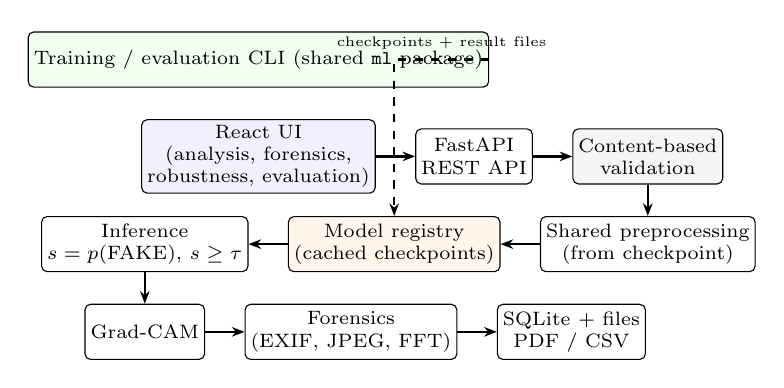
\begin{tikzpicture}[
  node distance=4mm and 5mm,
  box/.style={draw, rounded corners=2pt, align=center, font=\scriptsize, minimum height=7mm, inner sep=2pt, fill=white},
  arr/.style={-{Stealth[length=1.6mm]}, thick}]
\node[box, fill=blue!6] (ui) {React UI\\(analysis, forensics,\\robustness, evaluation)};
\node[box, right=of ui] (api) {FastAPI\\REST API};
\node[box, right=of api, fill=gray!8] (val) {Content-based\\validation};
\node[box, below=of val] (pre) {Shared preprocessing\\(from checkpoint)};
\node[box, left=of pre, fill=orange!8] (reg) {Model registry\\(cached checkpoints)};
\node[box, left=of reg] (inf) {Inference\\$s=p(\mathrm{FAKE})$, $s\ge\tau$};
\node[box, below=of inf] (cam) {Grad-CAM};
\node[box, right=of cam] (for) {Forensics\\(EXIF, JPEG, FFT)};
\node[box, right=of for] (db) {SQLite + files\\PDF / CSV};
\node[box, above=of ui, fill=green!6] (ml) {Training / evaluation CLI (shared \texttt{ml} package)};
\draw[arr] (ui) -- (api);
\draw[arr] (api) -- (val);
\draw[arr] (val) -- (pre);
\draw[arr] (pre) -- (reg);
\draw[arr] (reg) -- (inf);
\draw[arr] (inf) -- (cam);
\draw[arr] (cam) -- (for);
\draw[arr] (for) -- (db);
\draw[arr, dashed] (ml.east) -| node[pos=0.25, above, font=\tiny]{checkpoints + result files} (reg.north);
\end{tikzpicture}}
\caption{Platform architecture. Training, evaluation and the API share one \texttt{ml} package, so preprocessing is identical at training, evaluation and inference time.}
\label{fig:system}
\end{figure}

\subsection{Detector architecture}
Fig.~\ref{fig:detector} shows the detector. A backbone $f_\theta$ (ResNet-50 or EfficientNet-B0, initialised with torchvision ImageNet weights \cite{deng2009imagenet}) maps an input $x\in\mathbb{R}^{3\times224\times224}$ to a globally pooled feature vector $h=f_\theta(x)$ with $d=2048$ (ResNet-50) or $d=1280$ (EfficientNet-B0). The ImageNet classifier is replaced by dropout ($p=0.3$) and a linear layer producing logits $z=Wh+b\in\mathbb{R}^2$, with class 0 = REAL and class 1 = FAKE. The fake score is
\begin{equation}
s(x)=\mathrm{softmax}(z)_1=\frac{e^{z_1}}{e^{z_0}+e^{z_1}},
\end{equation}
and an image is labelled FAKE iff $s(x)\ge\tau$. The score is not interpreted as a calibrated probability. The ResNet-50 and EfficientNet-B0 detectors have 23.51\,M and 4.01\,M parameters, respectively.

\begin{figure}[!t]
\centering
\resizebox{\columnwidth}{!}{%
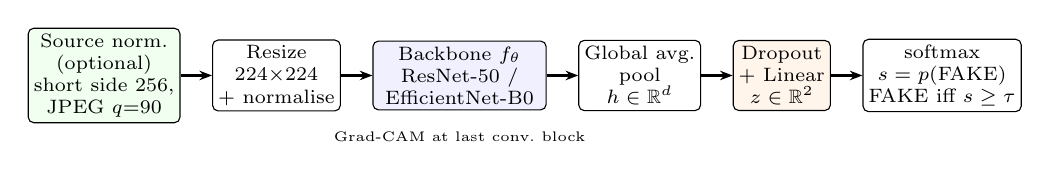
\begin{tikzpicture}[
  node distance=3.5mm and 4mm,
  box/.style={draw, rounded corners=2pt, align=center, font=\scriptsize, minimum height=8mm, inner sep=2pt},
  arr/.style={-{Stealth[length=1.6mm]}, thick}]
\node[box, fill=green!6] (src) {Source norm.\\(optional)\\short side 256,\\JPEG $q{=}90$};
\node[box, right=of src] (in) {Resize\\$224{\times}224$\\+ normalise};
\node[box, right=of in, fill=blue!6, minimum width=22mm] (bb) {Backbone $f_\theta$\\ResNet-50 /\\EfficientNet-B0};
\node[box, right=of bb] (gap) {Global avg.\\pool\\$h\in\mathbb{R}^{d}$};
\node[box, right=of gap, fill=orange!8] (head) {Dropout\\+ Linear\\$z\in\mathbb{R}^2$};
\node[box, right=of head] (sm) {softmax\\$s=p(\mathrm{FAKE})$\\FAKE iff $s\ge\tau$};
\node[font=\tiny, align=center, below=1.5mm of bb] (gc) {Grad-CAM at last conv.\ block};
\draw[arr] (src) -- (in);
\draw[arr] (in) -- (bb);
\draw[arr] (bb) -- (gap);
\draw[arr] (gap) -- (head);
\draw[arr] (head) -- (sm);
\end{tikzpicture}}
\caption{Detector pipeline. The ImageNet head is replaced by a two-class head; the decision threshold $\tau$ is selected on the validation split. The source normalisation is applied identically to every image in training, evaluation and inference.}
\label{fig:detector}
\end{figure}

\subsection{Preprocessing and source normalisation}
Images are decoded, converted to RGB, resized to $224\times224$ (bilinear) and normalised with ImageNet statistics. This transform is stored in each checkpoint and is used unchanged for validation, testing and API inference. Because all DFF fakes share one size and encoding (Sec.~\ref{sec:data}), we also evaluate a \emph{source normalisation}: each image, whatever its class, is first resized (bicubic) so that its shorter side is 256 pixels, centre-cropped to $256\times256$ and re-encoded as JPEG with quality 90. This removes the size and encoding difference between classes before the model sees any pixels.

\subsection{Training}\label{sec:training}
Models are fine-tuned with cross-entropy and AdamW \cite{loshchilov2019adamw}, using weight decay $10^{-4}$ and a learning rate of $10^{-4}$ for ResNet-50 and $3{\times}10^{-4}$ for EfficientNet-B0. The schedule is a one-epoch linear warm-up followed by cosine decay. We clip gradients at 1.0, use batch sizes of 48 and 64, and train with float16 automatic mixed precision on an NVIDIA GeForce RTX~4060 Laptop GPU (8\,GB). Augmentation consists of horizontal flips and random crops covering 80--100\% of the image area. Training uses a fixed, seeded, class-balanced random subset of 30{,}000 training images (15{,}000 per class). Model and threshold selection use a balanced subset of 6{,}000 validation images. Each model trains for 8 epochs with early stopping on validation ROC-AUC (patience 3); for all three models the best epoch was the last. The threshold $\tau$ maximises Youden's $J=\mathrm{TPR}-\mathrm{FPR}$ \cite{youden1950index} on the validation subset. The test split is never used for model or threshold selection. Software: PyTorch 2.14 \cite{paszke2019pytorch}, torchvision 0.29, scikit-learn 1.9; random seed 42.

\subsection{Explainability}
Grad-CAM \cite{selvaraju2017gradcam} computes $L^c=\mathrm{ReLU}(\sum_k\alpha_k^cA^k)$ with $\alpha_k^c=\frac{1}{Z}\sum_{i,j}\partial z_c/\partial A^k_{ij}$ over the feature maps $A^k$ of the last convolutional block. This is a $7\times7$ grid at $224^2$ input, computed for the predicted class $c$. We treat the maps as qualitative evidence only.

\subsection{Evaluation protocol}
We report accuracy, per-class precision and recall, macro-F1, ROC-AUC and confusion matrices, with FAKE as the positive class. We also report single-image latency (batch size 1, warm-up excluded, CUDA-synchronised). 95\% confidence intervals use a percentile bootstrap with 1{,}000 resamples over leakage groups rather than images \cite{efron1993bootstrap}. Resampling whole groups respects the correlation between a real image and the fakes derived from it. Robustness is measured at the unchanged threshold under JPEG compression (quality 90, 70 and 50), downscaling ($\times0.5$ and $\times0.25$, resized back to the original size), Gaussian blur ($\sigma=1,2$) and additive Gaussian noise ($\sigma=5,15$ on the 0--255 scale). Each perturbation is applied to the image file before the full preprocessing pipeline of the respective model. To measure generalisation to unseen manipulations, we retrain EfficientNet-B0 three times, each time removing one manipulation method from the training and validation data (threshold re-selected on the reduced validation set), and test on the 4{,}500 real test images plus 4{,}500 test images of the held-out method.

\section{Dataset and Data Audit}\label{sec:data}
DFF \cite{song2023dff} contains 30{,}000 real celebrity photographs from IMDB-WIKI \cite{rothe2018imdbwiki}. Each one has three fakes: Stable Diffusion inpainting, an InsightFace \cite{deng2019arcface} face swap, and Stable Diffusion v1.5 \cite{rombach2022ldm} text-to-image generation, for 120{,}000 images in total. Every fake is stored under the file name of its source photograph, which provides an initial leakage group (one real image and its three fakes).

Table~\ref{tab:audit} summarises the audit. No file was missing or corrupted. However, 165 sets (344 images) of byte-identical real photographs are filed under different identifiers, and no set mixes labels. With an identity-only split (v1), 84 of these sets and 19{,}949 cross-identity near-duplicate pairs (64-bit dHash, Hamming distance $\le4$) would span different splits. We therefore merge leakage groups connected by near-duplicates (Hamming $\le2$, union-find) before a 70/15/15 group-level split (v2, Table~\ref{tab:dataset}). This reduces 30{,}000 groups to 18{,}511. The perceptual hash can also merge similar but distinct faces, which only makes the split more conservative. The audit further showed that all 90{,}000 fakes are 512$\times$512 JPEGs while no real image is 512$\times$512. In a random sample of 3{,}000 real images the median short side is 440\,px (5th percentile 223\,px), and 1{,}048 real images are PNG, GIF or MPO files. All results use the v2 split. The test set is a class-balanced random sample of 4{,}500 real and 4{,}500 fake test images; the robustness suite uses a balanced random subset of 3{,}000 test images.

\begin{table}[!t]
\centering
\caption{Data audit of DeepFakeFace (DFF). v1: split by IMDB-WIKI id only; v2 (used for all results): groups merged across (near-)duplicates before splitting.}
\label{tab:audit}
\begin{tabular}{lr}
\toprule
Check & Result \\
\midrule
Images checked / missing / corrupted & 120,000 / 0 / 0 \\
Exact-duplicate sets (SHA-256) & 165 \\
\quad of which span splits (v1 split) & 84 \\
Near-duplicate pairs, dHash $\le$ 4 & 65,542 \\
\quad cross-group pairs spanning splits (v1) & 19,949 \\
Leakage groups before / after merging (dHash $\le$ 2) & 30,000 / 18,511 \\
Fake images that are 512$\times$512 JPEG & 100\% (90{,}000) \\
Real images that are 512$\times$512 & 0\% (0) \\
\bottomrule
\end{tabular}
\end{table}

\begin{table}[!t]
\centering
\caption{Dataset splits after leakage-aware grouping (all images; training uses a class-balanced random subset of the train split, see Sec.~\ref{sec:training}).}
\label{tab:dataset}
\begin{tabular}{llrrr}
\toprule
Dataset & Split & Real & Fake & Groups \\
\midrule
DFF (face) & train & 21,001 & 63,003 & 12,942 \\
 & val & 4,499 & 13,497 & 2,763 \\
 & test & 4,500 & 13,500 & 2,806 \\
\bottomrule
\end{tabular}
\end{table}


\section{Results}\label{sec:results}

\subsection{Detection performance}
Table~\ref{tab:main_dff} reports test performance. ResNet-50 reaches 95.12\% accuracy and 0.990 ROC-AUC, and EfficientNet-B0 reaches 94.38\% and 0.988. With source normalisation, EfficientNet-B0 reaches 95.47\% (95\% CI 94.99--95.89) and 0.991 ROC-AUC. Its accuracy interval does not overlap that of EfficientNet-B0 without normalisation (93.91--94.81). Normalisation therefore does \emph{not} reduce performance. This indicates that the size and format difference between classes is not the main cue the detector relies on, even though it is present in the data. The confidence intervals of ResNet-50 and normalised EfficientNet-B0 overlap, so we do not rank these two models. The validation-selected thresholds differ widely ($\tau=0.194$, $0.638$ and $0.337$), which shows that the default threshold of 0.5 is inappropriate for uncalibrated scores. EfficientNet-B0 trains faster than ResNet-50 (57--62\,s vs.\ 95\,s per epoch) with 5.9$\times$ fewer parameters, and all models classify an image in under 10\,ms. Fig.~\ref{fig:roc} shows the ROC curves and Table~\ref{tab:confusion} the confusion matrices.

\begin{table*}[!t]
\centering
\caption{Facial-deepfake detection on the DeepFakeFace test split. n = 9,000 test images (4,500 real / 4,500 fake); 95\% grouped-bootstrap CIs in brackets; threshold $\tau$ selected on validation; latency: batch size 1, RTX~4060, AMP.}
\label{tab:main_dff}
\setlength{\tabcolsep}{4pt}
\begin{tabular}{lccccccccc}
\toprule
 & Accuracy & \multicolumn{2}{c}{REAL} & \multicolumn{2}{c}{FAKE} & Macro & ROC-AUC & & Latency \\
\cmidrule(lr){3-4}\cmidrule(lr){5-6}
Model & (\%) & Prec. & Rec. & Prec. & Rec. & F1 & & $\tau$ & (ms) \\
\midrule
ResNet-50 & 95.12\,{\scriptsize[94.7, 95.6]} & 95.6 & 94.6 & 94.7 & 95.6 & 0.9512 & 0.9899\,{\scriptsize[0.988, 0.991]} & 0.194 & 6.9 \\
EfficientNet-B0 & 94.38\,{\scriptsize[93.9, 94.8]} & 92.6 & 96.4 & 96.3 & 92.3 & 0.9438 & 0.9879\,{\scriptsize[0.986, 0.989]} & 0.638 & 8.1 \\
EffNet-B0 + norm. & 95.47\,{\scriptsize[95.0, 95.9]} & 94.9 & 96.1 & 96.1 & 94.8 & 0.9547 & 0.9906\,{\scriptsize[0.989, 0.992]} & 0.337 & 7.6 \\
\bottomrule
\end{tabular}
\end{table*}

\begin{table}[!t]
\centering
\caption{Confusion matrices on the DFF test set (TN: real$\to$REAL, FP: real$\to$FAKE, FN: fake$\to$REAL, TP: fake$\to$FAKE).}
\label{tab:confusion}
\begin{tabular}{lrrrr}
\toprule
Model & TN & FP & FN & TP \\
\midrule
ResNet-50 & 4,257 & 243 & 196 & 4,304 \\
EfficientNet-B0 & 4,339 & 161 & 345 & 4,155 \\
EffNet-B0 + norm. & 4,325 & 175 & 233 & 4,267 \\
\bottomrule
\end{tabular}
\end{table}


\begin{figure}[!t]
\centering
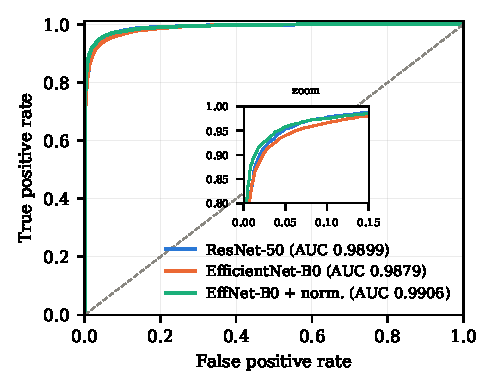
\includegraphics[width=\columnwidth]{generated/fig_roc_dff.pdf}
\caption{ROC curves on the DFF test split (inset: low false-positive region).}
\label{fig:roc}
\end{figure}

\subsection{Per-manipulation analysis}
Table~\ref{tab:per_method_dff} breaks performance down by manipulation. Without normalisation, fully generated and inpainted content is detected well (text-to-image 98.9--99.4\%, inpainting 95.6--98.3\%), but InsightFace swaps are the main source of errors (82.6\% for EfficientNet-B0, 89.3\% for ResNet-50). A face swap preserves most of the original photograph, so it leaves the least synthetic content to detect. Source normalisation raises face-swap detection to 91.4\% at the cost of slightly lower inpainting (94.9\%) and text-to-image (98.2\%) detection. Normalisation thus makes performance more uniform across manipulation types.

\begin{table}[!t]
\centering
\caption{Per-source accuracy (\%) on the DFF test split; mean fake score in parentheses. For fake sources accuracy equals the detection rate, for real images the specificity.}
\label{tab:per_method_dff}
\setlength{\tabcolsep}{3pt}
\begin{tabular}{lrccc}
\toprule
Source & n & ResNet-50 & EfficientNet-B0 & EffNet-B0 + norm. \\
\midrule
SD inpainting & 1,452 & 98.28 (0.961) & 95.59 (0.959) & 94.90 (0.936) \\
InsightFace swap & 1,519 & 89.34 (0.844) & 82.55 (0.843) & 91.38 (0.901) \\
SD v1.5 text2img & 1,529 & 99.41 (0.987) & 98.95 (0.989) & 98.17 (0.969) \\
Real (IMDB-WIKI) & 4,500 & 94.60 (0.040) & 96.42 (0.054) & 96.11 (0.037) \\
\bottomrule
\end{tabular}
\end{table}


\subsection{Robustness}
Table~\ref{tab:robust_dff} and Fig.~\ref{fig:robust} show that the unnormalised models are fragile. Mild JPEG compression (quality 90) is harmless. At quality 50, however, accuracy drops to 76.0\% (ResNet-50) and 74.2\% (EfficientNet-B0), mostly because real images are labelled fake (real-image recall 64.2\% and 66.3\%). Downscaling and blur have the same effect: at $\times0.25$, real-image recall falls to 69.1\% and 58.2\%, while fakes are still detected. Additive noise has the opposite effect. At $\sigma=15$, fake recall collapses to 10.1\% and 24.7\%, and almost every image is labelled real. These asymmetric failures show that the unnormalised detectors rely heavily on fine-grained, high-frequency image statistics. Any loss of detail looks ``fake'', and added noise makes an image look ``real''.

The normalised model is markedly more robust. Its mean accuracy over the nine perturbed conditions is 91.9\% (vs.\ 82.2\% and 81.4\%), its worst-case accuracy is 84.0\% (vs.\ 55.0\% and 61.9\%), and its accuracy stays at 90.7\% at JPEG quality 50. We attribute this to two properties of the normalisation. First, the model is trained only on images that were already resampled and JPEG-compressed, so it cannot depend on pristine compression artefacts. Second, the downsampling to 256 pixels acts as a low-pass filter that attenuates perturbations such as additive noise. Strong noise remains the most damaging condition (fake recall 69.7\%), which shows that the normalisation mitigates but does not remove the sensitivity.

\begin{table*}[!t]
\centering
\caption{Robustness on a balanced random subset of the DFF test set (n = 3,000). Perturbations are applied at test time; the model and validation-selected threshold are unchanged. Acc.\ and recalls in \%.}
\label{tab:robust_dff}
\setlength{\tabcolsep}{2.6pt}
\footnotesize
\begin{tabular}{lcccccccccccc}
\toprule
 & \multicolumn{4}{c}{ResNet-50} & \multicolumn{4}{c}{EfficientNet-B0} & \multicolumn{4}{c}{EffNet-B0 + norm.} \\
\cmidrule(lr){2-5}\cmidrule(lr){6-9}\cmidrule(lr){10-13}
Condition & Acc. & AUC & Rec.F & Rec.R & Acc. & AUC & Rec.F & Rec.R & Acc. & AUC & Rec.F & Rec.R \\
\midrule
Clean & 95.1 & 0.990 & 95.5 & 94.7 & 94.0 & 0.986 & 92.1 & 95.9 & 95.6 & 0.991 & 95.5 & 95.7 \\
JPEG q=90 & 94.7 & 0.990 & 95.1 & 94.4 & 93.9 & 0.984 & 92.4 & 95.4 & 95.8 & 0.991 & 95.6 & 96.0 \\
JPEG q=70 & 90.8 & 0.979 & 95.6 & 85.9 & 90.0 & 0.969 & 92.6 & 87.3 & 95.4 & 0.989 & 94.6 & 96.3 \\
JPEG q=50 & 76.0 & 0.878 & 87.8 & 64.2 & 74.2 & 0.845 & 82.1 & 66.3 & 90.7 & 0.964 & 88.7 & 92.7 \\
Downscale $\times$0.5 & 89.3 & 0.983 & 98.5 & 80.1 & 88.0 & 0.972 & 96.5 & 79.5 & 92.9 & 0.986 & 96.9 & 88.9 \\
Downscale $\times$0.25 & 82.9 & 0.951 & 96.6 & 69.1 & 78.2 & 0.945 & 98.1 & 58.2 & 91.4 & 0.976 & 93.4 & 89.4 \\
Blur $\sigma$=1.0 & 90.0 & 0.979 & 97.9 & 82.1 & 89.1 & 0.969 & 94.9 & 83.3 & 92.0 & 0.983 & 96.3 & 87.8 \\
Blur $\sigma$=2.0 & 87.6 & 0.952 & 90.3 & 84.9 & 84.2 & 0.945 & 94.7 & 73.7 & 89.6 & 0.971 & 94.1 & 85.0 \\
Noise $\sigma$=5.0 & 73.6 & 0.928 & 47.7 & 99.5 & 72.9 & 0.922 & 46.7 & 99.1 & 95.1 & 0.988 & 93.6 & 96.5 \\
Noise $\sigma$=15.0 & 55.0 & 0.811 & 10.1 & 99.9 & 61.9 & 0.830 & 24.7 & 99.1 & 84.0 & 0.958 & 69.7 & 98.3 \\
\midrule
\textit{Mean (perturbed)} & 82.2 & 0.939 & 80.0 & 84.5 & 81.4 & 0.931 & 80.3 & 82.4 & 91.9 & 0.978 & 91.4 & 92.3 \\
\textit{Worst case} & 55.0 & 0.811 & 10.1 & 64.2 & 61.9 & 0.830 & 24.7 & 58.2 & 84.0 & 0.958 & 69.7 & 85.0 \\
\bottomrule
\end{tabular}
\end{table*}


\begin{figure}[!t]
\centering
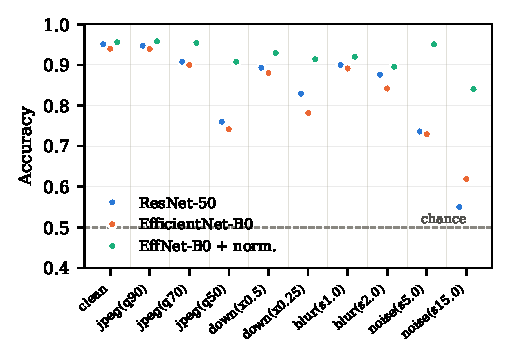
\includegraphics[width=\columnwidth]{generated/fig_robust_dff.pdf}
\caption{Test accuracy under perturbations (validation-selected thresholds unchanged). Each point is an independent condition; the dashed line marks chance level.}
\label{fig:robust}
\end{figure}

\subsection{Cross-manipulation generalisation}
Table~\ref{tab:cross_manip} shows that in-distribution accuracy does not transfer to unseen manipulations. When a method is held out, its detection rate drops from 99.0\% to 88.3\% for text-to-image faces, from 95.6\% to 39.2\% for inpainting and from 82.6\% to only 5.3\% for InsightFace swaps. The swap-held-out model is near chance overall (51.9\% accuracy), while real-image recall stays high (92.2--98.5\%), so the dominant error is that unseen fakes are accepted as real. ROC-AUC remains above chance (0.713--0.966), which indicates that a threshold tuned on the seen methods is particularly ill-suited to unseen ones. Fully synthetic faces share the most traces with the other diffusion-generated content and transfer best; face swaps, which keep most of the original photograph and are produced by a different pipeline, transfer worst. A detector trained on a fixed set of manipulations should therefore not be trusted on manipulation types it has not seen.

\begin{table*}[!t]
\centering
\caption{Cross-manipulation generalisation (EfficientNet-B0, no source normalisation). \emph{Seen}: detection rate when the method is in the training data (all methods trained jointly). \emph{Unseen}: the model is retrained without that method (train and validation) and tested on 4{,}500 real and 4{,}500 unseen-method test images (n = 9,000); 95\% grouped-bootstrap CIs in brackets. Rates in \%.}
\label{tab:cross_manip}
\setlength{\tabcolsep}{4pt}
\begin{tabular}{lccccc}
\toprule
 & \multicolumn{2}{c}{Fake detection rate} & \multicolumn{3}{c}{Held-out evaluation} \\
\cmidrule(lr){2-3}\cmidrule(lr){4-6}
Manipulation & Seen & Unseen & Real recall & Accuracy & ROC-AUC \\
\midrule
SD inpainting & 95.6 & 39.2 & 94.9 & 67.0\,{\scriptsize[66.3, 67.8]} & 0.844\,{\scriptsize[0.838, 0.850]} \\
InsightFace face swap & 82.6 & 5.3 & 98.5 & 51.9\,{\scriptsize[51.6, 52.3]} & 0.713\,{\scriptsize[0.706, 0.721]} \\
SD v1.5 text-to-image & 99.0 & 88.3 & 92.2 & 90.3\,{\scriptsize[89.6, 90.9]} & 0.966\,{\scriptsize[0.963, 0.969]} \\
\bottomrule
\end{tabular}
\end{table*}


\subsection{Explainability}
Fig.~\ref{fig:gradcam} shows Grad-CAM maps for randomly sampled true positives, true negatives, false positives and false negatives of ResNet-50. For fakes and many real images the maps concentrate on the face, whereas some false positives highlight clothing or background. The real class also contains non-portrait images (e.g.\ a postage stamp), which reveals label noise in the source data. False negatives receive very low fake scores ($s\approx0$), so the model fails with high confidence on some swaps and inpaintings. These maps are qualitative and do not establish that the model uses forensically meaningful evidence.

\begin{figure}[!t]
\centering
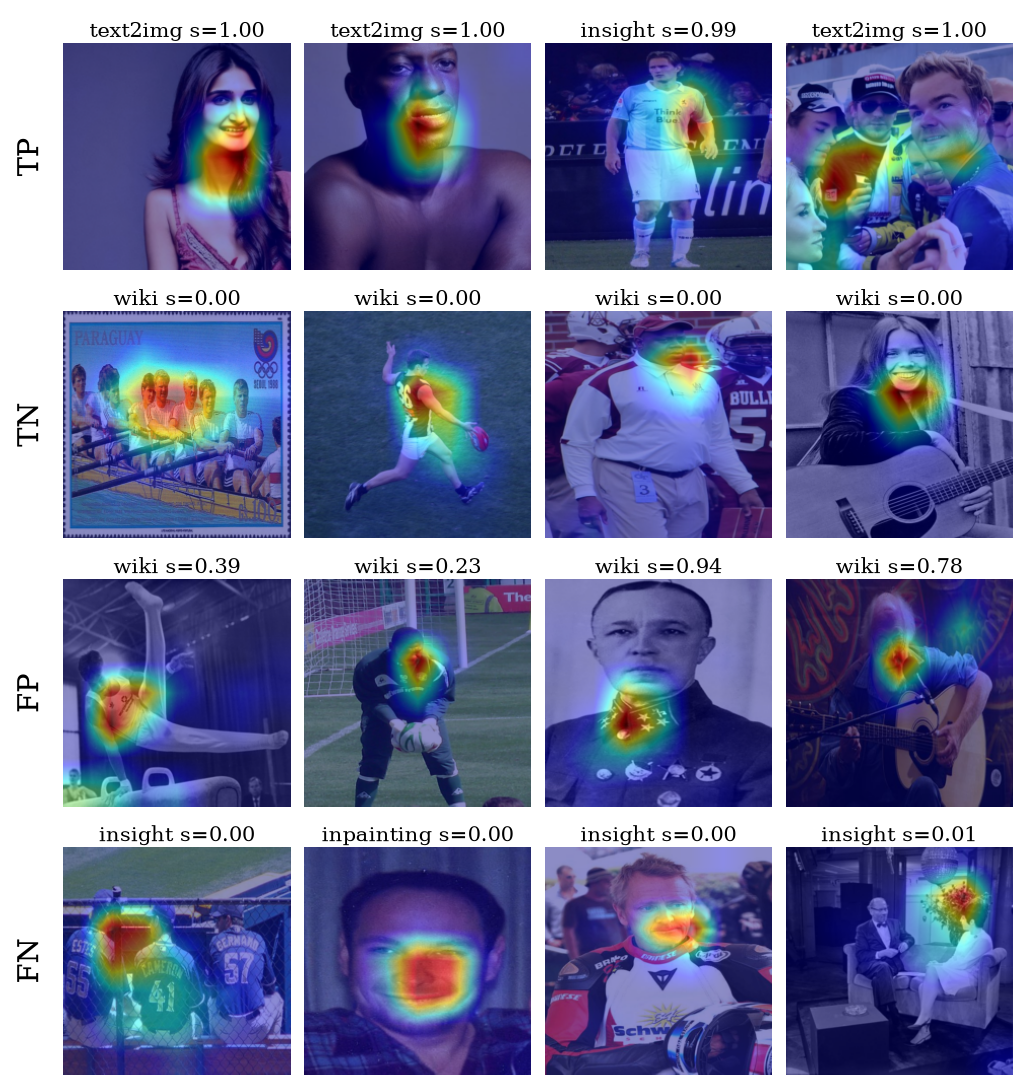
\includegraphics[width=\columnwidth]{generated/fig_gradcam_dff.png}
\caption{Grad-CAM (predicted class) for ResNet-50 on DFF test images. Rows: true positives, true negatives, false positives, false negatives; $s$ is the fake score ($\tau=0.194$).}
\label{fig:gradcam}
\end{figure}

\section{Discussion and Limitations}
Our results show that high in-distribution accuracy (about 95\%) can coexist with severe fragility to common post-processing and with poor transfer to unseen manipulation methods, and that a simple, label-agnostic normalisation of every input greatly reduces this fragility without loss of accuracy. We therefore recommend reporting detectors together with a data audit, leakage-aware splits, threshold provenance and a robustness suite. This study has several limitations:
\begin{itemize}
\item Each configuration was trained with a single seed. The confidence intervals capture test-set sampling variability, not training variability.
\item All experiments use one dataset; cross-manipulation tests were run for EfficientNet-B0 without source normalisation only, and generalisation to other face datasets was not evaluated.
\item The models are ImageNet-pretrained CNNs only.
\item The near-duplicate merging relies on a coarse perceptual hash.
\item The robustness perturbations are synthetic and applied one at a time.
\end{itemize}
The detector outputs a score, not proof. The platform therefore presents every prediction with its threshold, an uncertainty disclaimer and measured forensic context, and it performs no identity recognition.

\section{Conclusion}
We presented a leakage-aware evaluation of CNN detectors for diffusion-era facial deepfakes, integrated into an explainable forensic analysis platform. A data audit of DFF uncovered cross-identity duplicates and a systematic size and format difference between classes. After duplicate-aware splitting, ResNet-50 and EfficientNet-B0 reach 95.1\% and 94.4\% test accuracy but degrade to 55--76\% under strong compression or noise, and face swaps remain the hardest manipulation. Normalising every input to a common size and JPEG encoding yields 95.5\% accuracy, 91.4\% face-swap detection and 91.9\% mean accuracy under perturbations. However, detection of manipulation methods absent from training collapses (5.3\% for unseen face swaps, 39.2\% for unseen inpainting). Future work includes training for cross-manipulation generalisation, combining source normalisation with held-out-method evaluation, cross-dataset evaluation, multiple training seeds and calibrated uncertainty estimates.

\section*{Data and Code Availability}
DFF is available from its authors under its stated license. The manifests, configurations, result files, and the script that generates all tables and figures in this paper are part of the project repository.

\begin{thebibliography}{00}
\bibitem{rossler2019ff} A. R\"ossler, D. Cozzolino, L. Verdoliva, C. Riess, J. Thies, and M. Nie{\ss}ner, ``FaceForensics++: Learning to detect manipulated facial images,'' in \textit{Proc. IEEE/CVF Int. Conf. Comput. Vis. (ICCV)}, 2019, pp. 1--11.
\bibitem{song2023dff} H. Song, S. Huang, Y. Dong, and W.-W. Tu, ``Robustness and generalizability of deepfake detection: A study with diffusion models,'' arXiv:2309.02218, 2023.
\bibitem{he2016resnet} K. He, X. Zhang, S. Ren, and J. Sun, ``Deep residual learning for image recognition,'' in \textit{Proc. IEEE Conf. Comput. Vis. Pattern Recognit. (CVPR)}, 2016, pp. 770--778.
\bibitem{tan2019efficientnet} M. Tan and Q. V. Le, ``EfficientNet: Rethinking model scaling for convolutional neural networks,'' in \textit{Proc. Int. Conf. Mach. Learn. (ICML)}, 2019, pp. 6105--6114.
\bibitem{selvaraju2017gradcam} R. R. Selvaraju, M. Cogswell, A. Das, R. Vedantam, D. Parikh, and D. Batra, ``Grad-CAM: Visual explanations from deep networks via gradient-based localization,'' in \textit{Proc. IEEE Int. Conf. Comput. Vis. (ICCV)}, 2017, pp. 618--626.
\bibitem{wang2020cnn} S.-Y. Wang, O. Wang, R. Zhang, A. Owens, and A. A. Efros, ``CNN-generated images are surprisingly easy to spot\ldots for now,'' in \textit{Proc. IEEE/CVF Conf. Comput. Vis. Pattern Recognit. (CVPR)}, 2020, pp. 8695--8704.
\bibitem{ojha2023universal} U. Ojha, Y. Li, and Y. J. Lee, ``Towards universal fake image detectors that generalize across generative models,'' in \textit{Proc. IEEE/CVF Conf. Comput. Vis. Pattern Recognit. (CVPR)}, 2023, pp. 24480--24489.
\bibitem{corvi2023diffusion} R. Corvi, D. Cozzolino, G. Zingarini, G. Poggi, K. Nagano, and L. Verdoliva, ``On the detection of synthetic images generated by diffusion models,'' in \textit{Proc. IEEE Int. Conf. Acoust., Speech Signal Process. (ICASSP)}, 2023.
\bibitem{durall2020upconv} R. Durall, M. Keuper, and J. Keuper, ``Watch your up-convolution: CNN based generative deep neural networks are failing to reproduce spectral distributions,'' in \textit{Proc. IEEE/CVF Conf. Comput. Vis. Pattern Recognit. (CVPR)}, 2020, pp. 7890--7899.
\bibitem{frank2020frequency} J. Frank, T. Eisenhofer, L. Sch\"onherr, A. Fischer, D. Kolossa, and T. Holz, ``Leveraging frequency analysis for deep fake image recognition,'' in \textit{Proc. Int. Conf. Mach. Learn. (ICML)}, 2020, pp. 3247--3258.
\bibitem{grommelt2024fake} P. Grommelt, L. Weiss, F.-J. Pfreundt, and J. Keuper, ``Fake or JPEG? Revealing common biases in generated image detection datasets,'' arXiv:2403.17608, 2024.
\bibitem{rothe2018imdbwiki} R. Rothe, R. Timofte, and L. Van Gool, ``Deep expectation of real and apparent age from a single image without facial landmarks,'' \textit{Int. J. Comput. Vis.}, vol. 126, no. 2--4, pp. 144--157, 2018.
\bibitem{deng2019arcface} J. Deng, J. Guo, N. Xue, and S. Zafeiriou, ``ArcFace: Additive angular margin loss for deep face recognition,'' in \textit{Proc. IEEE/CVF Conf. Comput. Vis. Pattern Recognit. (CVPR)}, 2019, pp. 4690--4699.
\bibitem{rombach2022ldm} R. Rombach, A. Blattmann, D. Lorenz, P. Esser, and B. Ommer, ``High-resolution image synthesis with latent diffusion models,'' in \textit{Proc. IEEE/CVF Conf. Comput. Vis. Pattern Recognit. (CVPR)}, 2022, pp. 10684--10695.
\bibitem{deng2009imagenet} J. Deng, W. Dong, R. Socher, L.-J. Li, K. Li, and L. Fei-Fei, ``ImageNet: A large-scale hierarchical image database,'' in \textit{Proc. IEEE Conf. Comput. Vis. Pattern Recognit. (CVPR)}, 2009, pp. 248--255.
\bibitem{loshchilov2019adamw} I. Loshchilov and F. Hutter, ``Decoupled weight decay regularization,'' in \textit{Proc. Int. Conf. Learn. Represent. (ICLR)}, 2019.
\bibitem{youden1950index} W. J. Youden, ``Index for rating diagnostic tests,'' \textit{Cancer}, vol. 3, no. 1, pp. 32--35, 1950.
\bibitem{efron1993bootstrap} B. Efron and R. J. Tibshirani, \textit{An Introduction to the Bootstrap}. New York, NY, USA: Chapman \& Hall, 1993.
\bibitem{paszke2019pytorch} A. Paszke \textit{et al.}, ``PyTorch: An imperative style, high-performance deep learning library,'' in \textit{Adv. Neural Inf. Process. Syst. (NeurIPS)}, 2019, pp. 8024--8035.
\end{thebibliography}

\end{document}
